\documentclass{standalone}
\usepackage{tikz}
\usepackage{amssymb}
\usepackage{amsmath}
\usepackage{amstext}
\usepackage{xcolor}
\usetikzlibrary{positioning,shapes.geometric}
\usetikzlibrary{arrows}
\newcommand{\RN}[1]{%
  \textup{\uppercase\expandafter{\romannumeral#1}}%
}

\begin{document}

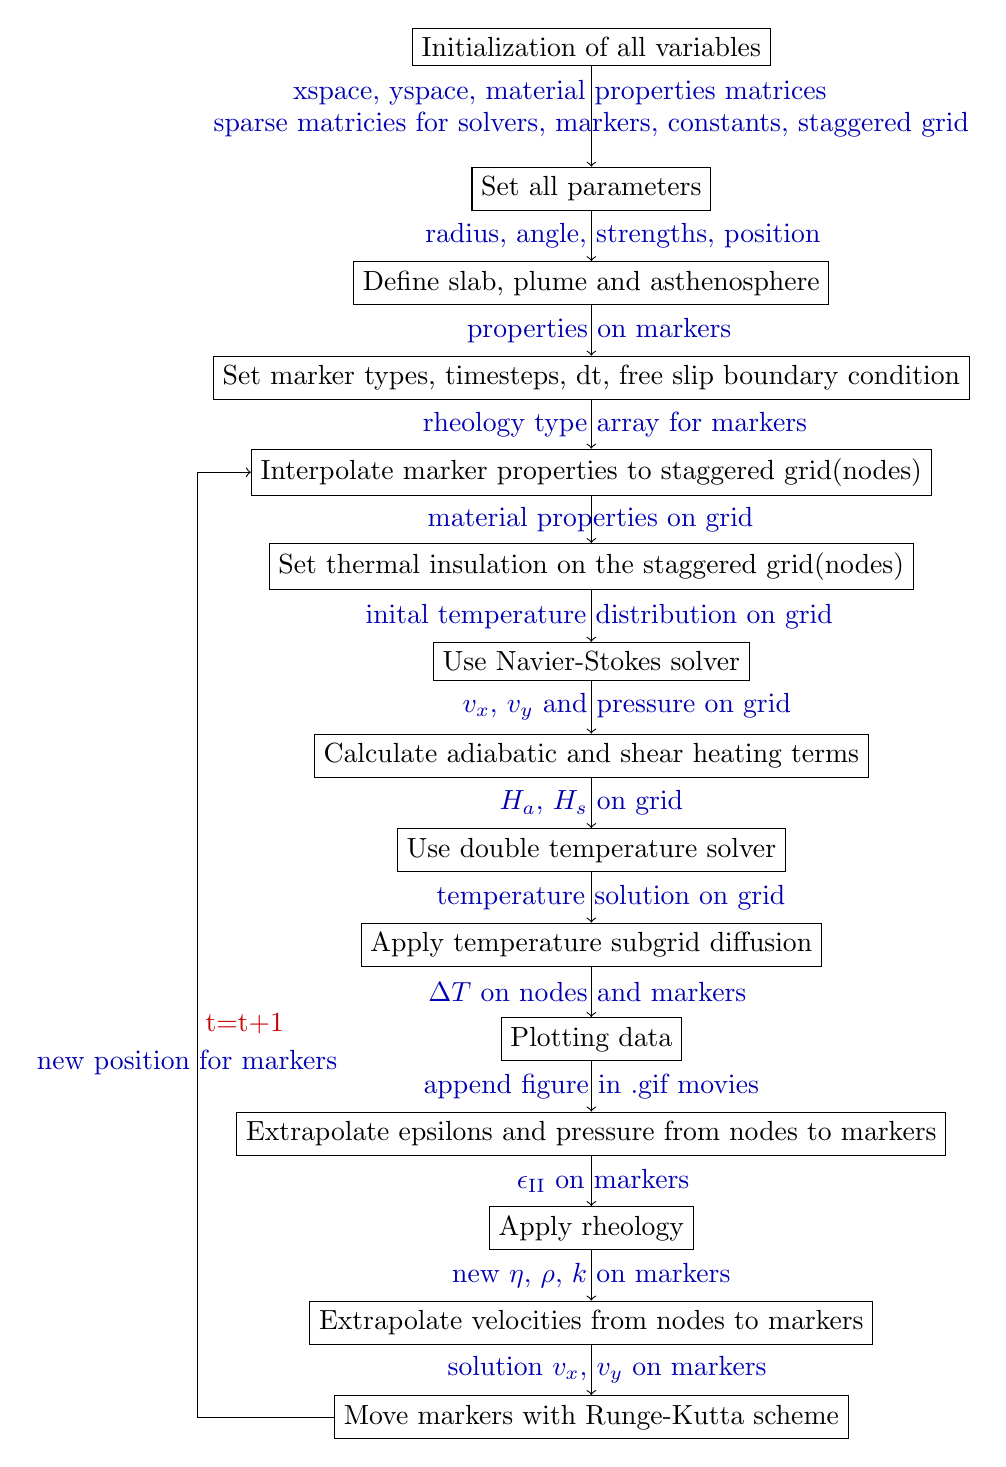
\begin{tikzpicture}[
	  scale=1.0,
	  %style for arrows
	  arrw/.style={thin, ->, >=to},
      % fisrt style for boxes      
      op/.style={rectangle, fill=black!15, draw=black},
      % second style for boxes
      dt/.style={rectangle, fill=white, draw=black,yshift=-0.2cm},
      cb/.style={color=blue!70!black}
      ]
            
      %nodes
      \node[dt](initdom){Initialization of all variables};
      \node[dt,below of=initdom,yshift=-0.6cm](setparams){Set all parameters};
      \node[dt,below of=setparams](geometry){Define slab, plume and asthenosphere};
      \node[dt,below of=geometry](markers){Set marker types, timesteps, dt, free slip boundary condition};
      
      \node[dt,below of=markers](startinterpol){Interpolate marker properties to staggered grid(nodes)};
      \node[dt,below of=startinterpol](deftemp){Set thermal insulation on the staggered grid(nodes)};
      \node[dt,below of=deftemp](navierstokes){Use Navier-Stokes solver};
      \node[dt,below of=navierstokes](heatingterms){Calculate adiabatic and shear heating terms};
      \node[dt,below of=heatingterms](tempsolver){Use double temperature solver};
      \node[dt,below of=tempsolver](tempdiff){Apply temperature subgrid diffusion};
      \node[dt,below of=tempdiff](fig){Plotting data};
      \node[dt,below of=fig](extrapolation){Extrapolate epsilons and pressure from nodes to markers};
      \node[dt,below of=extrapolation](rheology){Apply rheology};
      \node[dt,below of=rheology](extrapolvelocity){Extrapolate velocities from nodes to markers};
      \node[dt,below of=extrapolvelocity](rungekutta){Move markers with Runge-Kutta scheme};
      %edges
	  \draw[arrw](rungekutta) --node[cb,xshift=-1cm,yshift=4.5cm]{new position for markers} ++(-5,0)-| node[xshift=0.6cm,yshift=5.0cm,color=red!80!black]{t=t+1} ++(0,6)|- (startinterpol);
	  \draw[arrw](initdom)--node[cb,xshift=-0.4cm,yshift=0.3cm]{xspace, yspace, material properties matrices} node[cb,yshift=-0.1cm]{sparse matricies for solvers, markers, constants, staggered grid}(setparams);
	  \draw[arrw](setparams) -- node[cb,xshift=0.4cm]{radius, angle, strengths, position} (geometry);
	  \draw[arrw](geometry) --node[cb,xshift=0.1cm]{properties on markers} (markers);
	  \draw[arrw](markers) --node[cb,xshift=0.3cm]{rheology type array for markers} (startinterpol);
	  \draw[arrw](startinterpol)--node[cb,xshift=-0.01cm]{material properties on grid} (deftemp);
	  \draw[arrw](deftemp)--node[cb,xshift=0.1cm]{inital temperature distribution on grid} (navierstokes);
	  \draw[arrw](navierstokes)--node[cb,xshift=0.45cm]{$v_x$, $v_y$ and pressure on grid} (heatingterms);
	  \draw[arrw](heatingterms)--node[cb]{$H_a$, $H_s$ on grid} (tempsolver);
	  \draw[arrw](tempsolver) --node[cb,xshift=0.25cm]{temperature solution on grid} (tempdiff);
	  \draw[arrw](tempdiff) --node[cb,xshift=-0.05cm]{$\Delta T$ on nodes and markers} (fig);
	  \draw[arrw](fig) --node[cb]{append figure in .gif movies} (extrapolation);
	  \draw[arrw](extrapolation)--node[cb,xshift=0.15cm]{$\epsilon_{\RN{2}}$ on markers}(rheology);
	  \draw[arrw](rheology) --node[cb]{new $\eta$, $\rho$, $k$ on markers} (extrapolvelocity);
	  \draw[arrw](extrapolvelocity)--node[cb,xshift=0.2cm]{solution $v_x$, $v_y$ on markers}(rungekutta);
\end{tikzpicture}
  
\end{document}